\documentclass{article}[12pt]
\usepackage{fullpage,graphicx, setspace, latexsym, cite,amsmath,amssymb,xcolor,subfigure}
%\usepackage{epstopdf}
%\DeclareGraphicsExtensions{.pdf,.eps,.png,.jpg,.mps} 
\usepackage{amssymb} %maths
\usepackage{amsmath} %maths
\usepackage{amsthm, comment}
\usepackage[round,comma,sort, numbers]{natbib}

% \bibliographystyle{plain}
\bibliographystyle{plos2015}

\newtheorem{theorem}{Theorem}
\newtheorem{prop}{Proposition}
\newtheorem{corollary}{Corollary}
\newtheorem{lemma}{Lemma}
\newtheorem{defn}{Definition}
\newtheorem{ex}{Example}
\usepackage{float}

\newcommand*{\underuparrow}[1]{\underset{\uparrow}{#1}}
\usepackage{graphicx}
\usepackage{xcolor}
\usepackage[dvipsnames]{xcolor}
\usepackage{algorithmicx}
\usepackage{algorithm} %http://ctan.org/pkg/algorithms
\usepackage{algpseudocode} %http://ctan.org/pkg/algorithmicx
\usepackage{enumitem}
\usepackage{simplemargins}
\usepackage{hyperref}

\renewcommand{\bibnumfmt}[1]{#1.}
\setlist{noitemsep} % or \setlist{noitemsep} to leave space around whole list
\setallmargins{1in}
\linespread{1.1}


\def\R{\mathbb{R}}
\def\Eps{\mathcal{E}}
\def\E{\mathbb{E}}
\def\V{\mathbb{V}}
\def\F{\mathcal{F}}
\def\G{\mathcal{G}}
\def\H{\mathcal{H}}
\def\S{\mathcal{S}}
\def\P{\mathbb{P}}
\def\1{\mathbf{1}}
\def\n{\nappa}
\def\h{\mathbf{w}}
\def\v{\mathbf{v}}
\def\x{\mathbf{x}}
\def\X{\mathcal{X}}
\def\Y{\mathcal{Y}}
\def\eps{\epsilon}
\def\y{\mathbf{y}}
\def\e{\mathbf{e}}
\newcommand{\norm}[1]{\left|\left|#1\right|\right|}
\DeclareMathOperator*{\argmin}{arg\,min}
\DeclareMathOperator*{\argmax}{arg\,max}
\newcommand{\lecture}[4]{
   \pagestyle{myheadings}
   \thispagestyle{plain}
   \newpage
   % \setcounter{lecnum}{#1}
   \setcounter{page}{1}
   \setlength{\headsep}{10mm}
   \noindent
   \begin{center}
   \framebox{
      \vbox{\vspace{2mm}
    \hbox to 6.28in { {\bf CHEME 5820: Machine Learning for Engineers
   \hfill Spring 2025} }
       \vspace{4mm}
       \hbox to 6.28in { {\Large \hfill Lecture #1: #2  \hfill} }
       \vspace{2mm}
       \hbox to 6.28in { {\it Lecturer: #3 \hfill #4} }
      \vspace{2mm}}
   }
   \end{center}
   \markboth{Lecture #1: #2}{Lecture #1: #2}

   \noindent{\bf Disclaimer}: {\it These notes have not been subjected to the
   usual scrutiny reserved for formal publications. }
   \vspace*{4mm}
}


\begin{document}
\lecture{3a}{Linear Regression, Perceptron and Binary Classification}{Jeffrey Varner}{}

\section{Introduction}
In this lecture, we will introduce the perceptron algorithm for binary classification problems. 
The perceptron is a simple linear classifier that can be used to separate two classes of data points. 
The perceptron algorithm is a simple iterative algorithm that incrementally updates the weights of the linear classifier to minimize the classification error. 
We will first introduce the perceptron algorithm and then discuss its convergence properties, i.e., when the algorithm converges to a solution and when it does not.
The key concepts covered in this lecture include:
\begin{itemize}[leftmargin=16pt]
    \item{\textbf{Linear regression models}: A class of models used in machine learning for regression tasks, i.e., predicting a continuous output variable from one or more continuous or discrete input features. 
    Linear regression models assume that the output variable is a linear combination of the input features.}
    \item{\textbf{Binary classification}: The problem of classifying data points into one of two classes. Binary classification is a type of supervised machine learning task that involves categorizing data points into one of two distinct classes based on their features.
    These features can be continuous or discrete, and the classes can be represented as binary labels, e.g., $\{-1,1\}$ or $\{0,1\}$.}
    \item{\textbf{Perceptron}: The perceptron algorithm for binary classification problems is a linear classifier that separates two classes of data points. The perceptron algorithm is an iterative algorithm that incrementally updates the weights of the linear classifier to minimize the classification error.
    The perceptron algorithm is guaranteed to converge to a solution with no mistakes in a finite number of iterations if the data set is linearly separable. However, if the data set is not linearly separable, the perceptron algorithm will not converge to a perfect solution, but rather to a solution with some classification errors.}
\end{itemize}

\section{Linear Regression Models}
Linear regression models are a class of models used in machine learning for regression tasks, i.e., predicting a continuous output variable from one or more continous or discrete input features.
Linear regression models assume that the output variable is a linear combination of the input features, i.e., the output variable is a linear function of the input features.
Linear in this context is a misnomer in the sense that the features are not necessarily linear, but the model is linear in the parameters and the features.
Suppose we have a data set $\mathcal{D} = \left\{(\mathbf{x}_{1},y_{1}),\dotsc,(\mathbf{x}_{m},y_{m})\right\}$ with $m$ examples, where each example where $\mathbf{x}_{i}\in\R^{n}$ is a feature vector and $y_{i}\in\R$ is the output variable.
The linear regression model predicts the output variable $y_{i}$ for feature vector $\mathbf{x}_{i}$ using the linear function:
\begin{equation*}
    y_{i} = \mathbf{x}_{i}^{T}\cdot\beta + \epsilon_{i}
\end{equation*}
where we have augmented the feature vector $\mathbf{x}_{i}$ with a bias term, i.e., $\mathbf{x}_{i}^{T} = \left(x^{(i)}_{1},\dots,x^{(i)}_{n},1\right)$, $\beta = \left(w_{1},\dots,w_{n},b\right)$ is a column vector of (unknown) parameters $w_{j}\in\R$ corresponding to the importance (weight) of feature $j$ and a bias parameter $b\in\R$
and $\epsilon_{i}\sim\mathcal{N}(0,\sigma^{2})$ is a noise term, typically assumed to be a Normal distribution with mean zero and variance $\sigma^{2}$.
Depending upon the shape of the data and various other problem constraints, there are analytical solutions to for linear regression parameter vecrtoe $\beta$, e.g., the normal equations, or iterative solutions, e.g., gradient descent can be used to estimate the parameters $\beta$ for other linear regression problems.

\subsection{Overdetemined Linear Regression models}
If the number of examples $m$ is greater than the number of features $n$, the linear regression model is said to be overdetermined.
In other words, there are more examples than features.  Regularized linear regression models incorporate penalty terms to constrain the size of the coefficient estimates, thereby reducing overfitting and enhancing the model's generalizability to new data. 
Consider an overdetermined data matrix $\mathbf{X}\in\mathbb{R}^{m\times{n}}$, i.e., the case where $m>n$ (more examples than unknown parameters).
A regularized least squares estimate of the unknown parameters $\mathbf{\beta}$ for an overdetermined system will minimize a loss (objective) function of the form:
\begin{equation*}
\hat{\mathbf{\beta}}_{\lambda} = \arg\min_{\mathbf{\beta}} ||~\mathbf{y} - \mathbf{X}\cdot\mathbf{\beta}~||^{2}_{2} + \lambda\cdot||~\mathbf{\beta}~||^{2}_{2}
\end{equation*}
where $||\star||^{2}_{2}$ is the square of the $l2$-vector norm, $\lambda\geq{0}$ denotes a regularization parameter, and $\hat{\mathbf{\beta}}_{\lambda}$ denotes the estimated parameter vector. 
The parameters $\hat{\mathbf{\beta}}_{\lambda}$ that minimize the $||\star||^{2}_{2}$ loss plus penalty for overdetermined data matrix $\mathbf{X}$ are given by:
\begin{equation*}
\hat{\mathbf{\beta}}_{\lambda} = \left(\mathbf{X}^{T}\mathbf{X}+\lambda\cdot\mathbf{I}\right)^{-1}\mathbf{X}^{T}\mathbf{y} - \left(\mathbf{X}^{T}\mathbf{X}+\lambda\cdot\mathbf{I}\right)^{-1}\mathbf{X}^{T}\mathbf{\epsilon}
\end{equation*}
The matrix $\mathbf{X}^{T}\mathbf{X}+\lambda\cdot\mathbf{I}$ is the $\texttt{regularized normal matrix}$, while $\mathbf{X}^{T}\mathbf{y}$ is the $\texttt{moment vector}$. 
The inverse $\left(\mathbf{X}^{T}\mathbf{X}+\lambda\cdot\mathbf{I}\right)^{-1}$ must exist to obtain the estimated parameter vector $\hat{\mathbf{\beta}}_{\lambda}$.

\subsection{Underdetermined Linear Regression models}
Assume the data matrix $\mathbf{X}$ is $\texttt{underdetermined}$, i.e., $m < n$ (more columns than rows), and 
the error vector $\mathbf{\epsilon}\sim\mathcal{N}(\mathbf{0},\sigma^{2}\cdot\mathbf{I})$.
Then, an \href{https://en.wikipedia.org/wiki/Ordinary_least_squares}{ordinary least squares} estimate of the unknown parameters is the $\textit{smallest}$ parameter vector $\beta$ that satisfies the original equations:
\begin{eqnarray*}
\text{minimize}~& & ||\,\mathbf{\beta}\,|| \\
\text{subject to} & & \mathbf{X}\cdot\mathbf{\beta} = \mathbf{y}
\end{eqnarray*}
The least-norm problem has an analytical estimate for the unknown parameter vector $\hat{\mathbf{\beta}}$ given by:
\begin{equation*}
\hat{\mathbf{\beta}} =\mathbf{X}^{T}\left(\mathbf{X}\mathbf{X}^{T}\right)^{-1}\cdot\mathbf{y} - \mathbf{X}^{T}\left(\mathbf{X}\mathbf{X}^{T}\right)^{-1}\cdot\mathbf{\epsilon}
\end{equation*}
where inverse $\left(\mathbf{X}\mathbf{X}^{T}\right)^{-1}$ must exist to obtain the estimated model parameter vectors $\hat{\mathbf{\beta}}$.

\section{The Perceptron and Binary Classification}
The Perceptron \cite{Perceptron1960} is a simple yet powerful algorithm used in machine learning for binary classification tasks.
\href{https://en.wikipedia.org/wiki/Perceptron}{The Perceptron (Rosenblatt, 1957)} takes the (scalar) output of a linear regression model $y_{i}\in\mathbb{R}$ and transforms it, using a transform function $\sigma(\star) = \text{sign}(\star)$, into a discrete value representing a category, e.g., $\sigma:\mathbb{R}\rightarrow\{-1,1\}$ in the binary classification case. 
Suppose there exists a data set $\mathcal{D} = \left\{(\mathbf{x}_{1},y_{1}),\dotsc,(\mathbf{x}_{m},y_{m})\right\}$ with $m$ \textit{labeled} examples, where each example $1,2,\dots,m$ has been labeled by an expert, i.e., a human to be in a category $\hat{y}_{i}\in\{-1,1\}$, given the feature vector $\mathbf{x}_{i}\in\mathbb{R}^{n}$. 
The Perceptron \textit{incrementally} learns a linear decision boundary between two classes of possible objects (binary classification) in $\mathcal{D}$ by repeatedly processing the data. 
During each pass, a regression parameter vector $\mathbf{\beta}$ is updated until it makes no more than a specified number of mistakes. 

The Perceptron computes the label $\hat{y}_{i}$ for feature vector $\mathbf{x}_{i}$ using the $\sigma(\star) = \text{sign}(\star)$ function:
\begin{equation*}
    \hat{y}_{i} = \text{sign}\left(\mathbf{x}_{i}^{T}\cdot\beta\right)
\end{equation*}
where $\beta=\left(w_{1},\dots,w_{n}, b\right)$ is a column vector of (unknown) weight parameters $w_{j}\in\mathbb{R}$ corresponding to the importance of feature $j$ and a   bias parameter $b\in\mathbb{R}$, the features $\mathbf{x}^{T}_{i}=\left(x^{(i)}_{1},\dots,x^{(i)}_{n}, 1\right)$ is the $n+1$-dimensional feature (row) vector (features augmented with bias term), and $\text{sign}(z)$ is the $\texttt{sign}$ function:
\begin{equation*}
    \text{sign}(z) = 
    \begin{cases}
        1 & \text{if}~z\geq{0}\\
        -1 & \text{if}~z<0
    \end{cases}
\end{equation*}
If data set $\mathcal{D}$ is linearly separable, the Perceptron will find a separating hyperplane in a finite number of passes 
through $\mathcal{D}$. However, if the data set $\mathcal{D}$ is not linearly separable, the Perceptron will not converge.
Pusedo code for the perceptron algorithm is shown in Algorithm~\ref{alg:perceptron}.
\begin{algorithm}[H]
    \caption{The Perceptron Algorithm}\label{alg:perceptron}
    \begin{algorithmic}[1]
        % \Procedure{Incremental-Training-Perceptron}{$\mathcal{D}$}
        \State \textbf{Input:} $\mathcal{D} = \left\{(\mathbf{x}_{1},y_{1}),\dotsc,(\mathbf{x}_{m},y_{m})\right\}$, tolerance $\epsilon\geq{0}$, maximum iterations $\texttt{maxiter}$
        \State \textbf{Features:} $\mathbf{x}_{i} = \left(x_{i1},\dots, x_{in},1\right)$ are augmented with a bias term, labels $y_{i}\in\{-1,1\}$.
        \State \textbf{Output:} Classifier parameters $\mathbf{\beta} = \left(w_{1},\dots, w_{n}, b\right)$
        \State $\mathbf{\beta} \gets \texttt{rand}$\Comment{Initialize parameter vector $\mathbf{\beta}$ to a random vector}
        \State $i \gets 0$\Comment{Initialize the loop counter to zero}
        \While{$\text{true}$}\Comment{Repeat until stopping criterion is met}
        \State $\text{error} \gets 0$\Comment{Initialize the error count to zero for this pass through $\mathcal{D}$}
        \For{$(\mathbf{x},y)\in\mathcal{D}$}\Comment{Iterate over each pair $(\mathbf{x},y)$ in data set $\mathcal{D}$}
            \If{$y\cdot\left(\mathbf{x}^{T}\cdot\mathbf{\beta}\right) \leq 0$}\Comment{Ooops! The data pair $(\mathbf{x},y)$ is misclassified}
                \State $\mathbf{\beta} \gets \mathbf{\beta} + {y}\cdot\mathbf{x}$\Comment{Update the weight vector $\mathbf{\beta}$}
                \State $\text{error} \gets \text{error} + 1$\Comment{Increment the error count}
            \EndIf
        \EndFor
        \If{$\text{error} \leq \epsilon$ \textbf{or} $i\geq\texttt{maxiter}$ }\Comment{Stopping criterion: tolerance or max iterations?}
            \State \textbf{break} \Comment{Exit the training loop}    
        \EndIf
        \State $i \gets i + 1$\Comment{Increment the loop counter and repeat}
        \EndWhile
        % \EndProcedure
    \end{algorithmic}
\end{algorithm}

\section{Evaluation of the Binary Classifier}
Once the Perceptron (or any binary classifier) has converged, we can evaluate the performance of the binary classifier using a variety of metrics.
See Sidey-Gibbon et al \cite{SG2019} for a detailed discussion of these metrics in the context of medical classification problems.
The central idea is to compare the predicted labels $\hat{y}_{i}$ to the true labels $y_{i}$ in the data set $\mathcal{D}$. 
There are a variety of metrics that can be used to evaluate the performance of a binary classifier, but they all start with computing the confusion matrix.

\begin{figure}
    \centering
	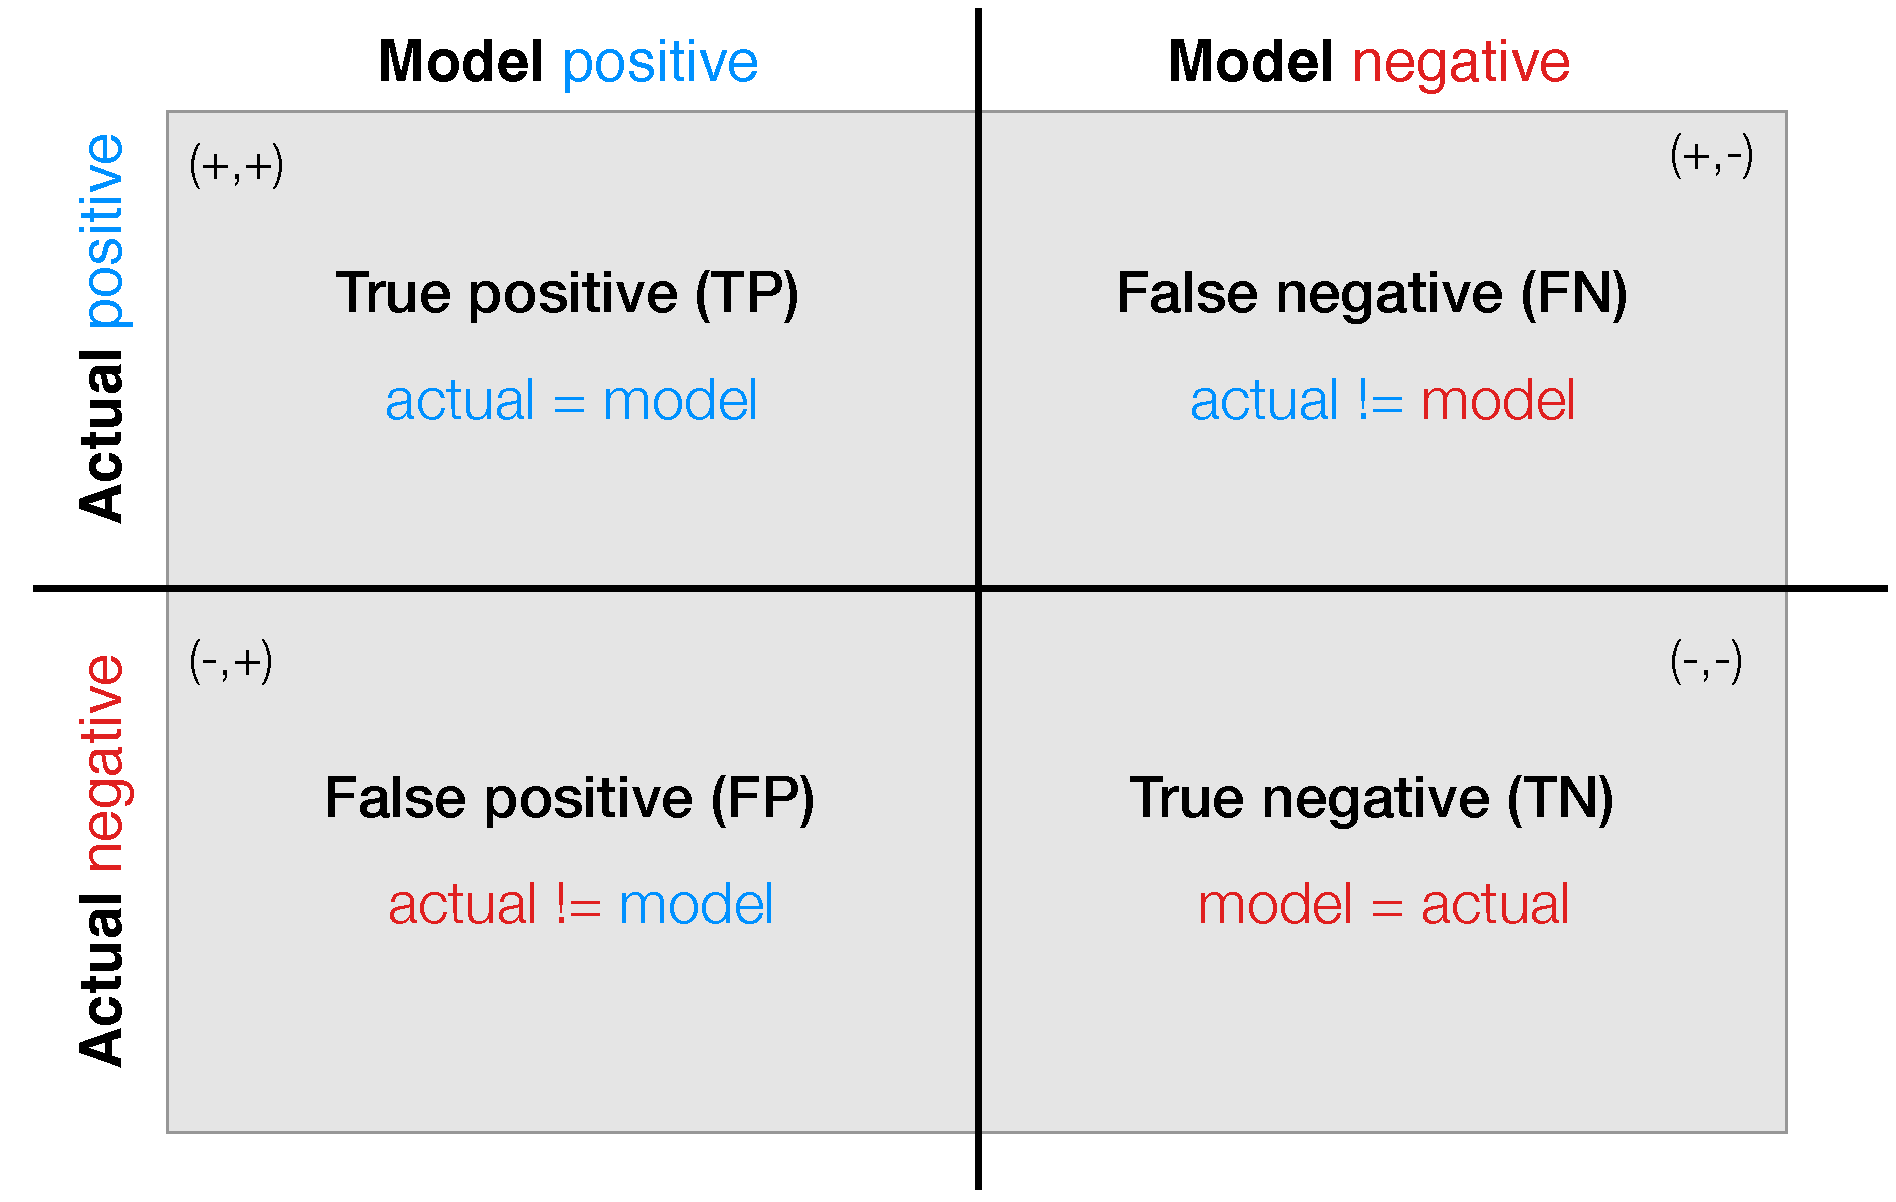
\includegraphics[width=0.75\textwidth]{./figs/Fig-BinaryConfusionMatrix.pdf}
	\caption{Confusion matrix schematic for the binary classification problem.}\label{fig:binaryconfusionmatrx}
\end{figure}

\subsection{Confusion Matrix}
The confusion matrix is a table that is often used to describe the performance of a classification model on a set of data for which the true values are known (Fig. \ref{fig:binaryconfusionmatrx}).
The confusion matrix is a $2\times{2}$ matrix that contains four entries: true positive (TP), false positive (FP), true negative (TN), and false negative (FN).
The true positive (TP) entry in the confusion matrix is the number of positive examples that were correctly classified as positive.
The false negative (FN) entry is the number of positive examples that were incorrectly classified as negative by the model.
The false positive (FP) entry is the number of negative examples that were incorrectly classified as positive by the model.
The true negative (TN) entry is the number of negative examples that were correctly classified as negative by the model.
The confusion matrix is used to calculate a variety of performance metrics, including accuracy, precision, recall, and the F1 score.

\paragraph*{Accuracy.}
The accuracy of a binary classifier is the proportion of correctly classified \textit{total} examples in the data set.
The accuracy is calculated as the sum of the true positive and true negative entries in the confusion matrix divided by the total number of examples in the data set:
\begin{equation*}
    \text{Accuracy} = \frac{TP + TN}{TP + TN + FP + FN}
\end{equation*}
Thus, accuracy is a measure of the overall performance of the classifier and indicates how well the classifier is able to correctly classify examples (both positive and negative).

\paragraph*{Precision.}
The precision of a binary classifier is the proportion of correctly classified \textit{positive} examples out of all examples that were classified as positive by the model.
The precision is calculated as the true positive entry in the confusion matrix divided by the sum of the true positive and false positive entries:
\begin{equation*}
    \text{Precision} = \frac{TP}{TP + FP}
\end{equation*}
Precision is a measure of the classifier's ability to correctly classify positive examples and is useful when the cost of false positives is high.

\paragraph*{Recall (Sensitivity).}
The recall of a binary classifier is the proportion of correctly classified \textit{positive} examples out of all examples that are truly positive in the data set.
The recall is calculated as the true positive entry in the confusion matrix divided by the sum of the true positive and false negative entries:
\begin{equation*}
    \text{Recall} = \frac{TP}{TP + FN}
\end{equation*}
Recall is a measure of the classifier's ability to correctly classify positive examples and is useful when the cost of false negatives is high.

\paragraph*{F1 Score.}
The F1 score of a binary classifier is the harmonic mean of precision and recall. The F1 score is calculated as:
\begin{equation*}
    \text{F1 Score} = 2\cdot\frac{\text{Precision}\cdot\text{Recall}}{\text{Precision} + \text{Recall}}
\end{equation*}
The F1 score is a measure of the classifier's overall performance and balances the trade-off between precision and recall.

\section{Summary}
In this lecture, we introduced the perceptron algorithm for binary classification problems.
The perceptron is a simple linear classifier that can be used to separate two classes of data points.
The perceptron algorithm is a simple iterative algorithm that incrementally updates the weights of the linear classifier to minimize the classification error.
Thus, it is one of the first examples of on online learning algorithm, i.e., an algorithm that learns from data in an incremental fashion.
The perceptron algorithm is guaranteed to converge to a solution if the data set is linearly separable.
However, if the data set is not linearly separable, the perceptron algorithm will not converge to a perfect solution.
If we are willing to accept some classification errors, we can use the perceptron algorithm to find a separating hyperplane in a finite number of passes through the data set, 
even if the data set is not linearly separable.

\bibliography{References-L3a.bib}

\end{document}